% Options for packages loaded elsewhere
\PassOptionsToPackage{unicode}{hyperref}
\PassOptionsToPackage{hyphens}{url}
%
\documentclass[
]{article}
\usepackage{lmodern}
\usepackage{amsmath}
\usepackage{ifxetex,ifluatex}
\ifnum 0\ifxetex 1\fi\ifluatex 1\fi=0 % if pdftex
  \usepackage[T1]{fontenc}
  \usepackage[utf8]{inputenc}
  \usepackage{textcomp} % provide euro and other symbols
  \usepackage{amssymb}
\else % if luatex or xetex
  \usepackage{unicode-math}
  \defaultfontfeatures{Scale=MatchLowercase}
  \defaultfontfeatures[\rmfamily]{Ligatures=TeX,Scale=1}
\fi
% Use upquote if available, for straight quotes in verbatim environments
\IfFileExists{upquote.sty}{\usepackage{upquote}}{}
\IfFileExists{microtype.sty}{% use microtype if available
  \usepackage[]{microtype}
  \UseMicrotypeSet[protrusion]{basicmath} % disable protrusion for tt fonts
}{}
\makeatletter
\@ifundefined{KOMAClassName}{% if non-KOMA class
  \IfFileExists{parskip.sty}{%
    \usepackage{parskip}
  }{% else
    \setlength{\parindent}{0pt}
    \setlength{\parskip}{6pt plus 2pt minus 1pt}}
}{% if KOMA class
  \KOMAoptions{parskip=half}}
\makeatother
\usepackage{xcolor}
\IfFileExists{xurl.sty}{\usepackage{xurl}}{} % add URL line breaks if available
\IfFileExists{bookmark.sty}{\usepackage{bookmark}}{\usepackage{hyperref}}
\hypersetup{
  pdftitle={Surgical sutures},
  pdfauthor={Andrew J. Sims},
  hidelinks,
  pdfcreator={LaTeX via pandoc}}
\urlstyle{same} % disable monospaced font for URLs
\usepackage[margin=1in]{geometry}
\usepackage{longtable,booktabs}
\usepackage{calc} % for calculating minipage widths
% Correct order of tables after \paragraph or \subparagraph
\usepackage{etoolbox}
\makeatletter
\patchcmd\longtable{\par}{\if@noskipsec\mbox{}\fi\par}{}{}
\makeatother
% Allow footnotes in longtable head/foot
\IfFileExists{footnotehyper.sty}{\usepackage{footnotehyper}}{\usepackage{footnote}}
\makesavenoteenv{longtable}
\usepackage{graphicx}
\makeatletter
\def\maxwidth{\ifdim\Gin@nat@width>\linewidth\linewidth\else\Gin@nat@width\fi}
\def\maxheight{\ifdim\Gin@nat@height>\textheight\textheight\else\Gin@nat@height\fi}
\makeatother
% Scale images if necessary, so that they will not overflow the page
% margins by default, and it is still possible to overwrite the defaults
% using explicit options in \includegraphics[width, height, ...]{}
\setkeys{Gin}{width=\maxwidth,height=\maxheight,keepaspectratio}
% Set default figure placement to htbp
\makeatletter
\def\fps@figure{htbp}
\makeatother
\setlength{\emergencystretch}{3em} % prevent overfull lines
\providecommand{\tightlist}{%
  \setlength{\itemsep}{0pt}\setlength{\parskip}{0pt}}
\setcounter{secnumdepth}{-\maxdimen} % remove section numbering
\ifluatex
  \usepackage{selnolig}  % disable illegal ligatures
\fi
\newlength{\cslhangindent}
\setlength{\cslhangindent}{1.5em}
\newlength{\csllabelwidth}
\setlength{\csllabelwidth}{3em}
\newenvironment{CSLReferences}[2] % #1 hanging-ident, #2 entry spacing
 {% don't indent paragraphs
  \setlength{\parindent}{0pt}
  % turn on hanging indent if param 1 is 1
  \ifodd #1 \everypar{\setlength{\hangindent}{\cslhangindent}}\ignorespaces\fi
  % set entry spacing
  \ifnum #2 > 0
  \setlength{\parskip}{#2\baselineskip}
  \fi
 }%
 {}
\usepackage{calc}
\newcommand{\CSLBlock}[1]{#1\hfill\break}
\newcommand{\CSLLeftMargin}[1]{\parbox[t]{\csllabelwidth}{#1}}
\newcommand{\CSLRightInline}[1]{\parbox[t]{\linewidth - \csllabelwidth}{#1}\break}
\newcommand{\CSLIndent}[1]{\hspace{\cslhangindent}#1}

\title{Surgical sutures}
\author{Andrew J. Sims}
\date{February 2021}

\begin{document}
\maketitle

\hypertarget{introduction}{%
\section{Introduction}\label{introduction}}

Leaper \emph{et al} {[}1{]} presented a model that compared
antimicrobial surgical sutures (absorbable sutures impregnated with
triclosan, TCS) with standard care, absorbable sutures with no
antimicrobial impregnation (NCS). The model was evaluated in three
scenarios:

\begin{itemize}
\tightlist
\item
  clean wounds;
\item
  clean-contaminated wounds;
\item
  contaminated and dirty wounds
\end{itemize}

\hypertarget{scenario-1-clean-wounds}{%
\section{Scenario 1: clean wounds}\label{scenario-1-clean-wounds}}

\begin{figure}

{\centering 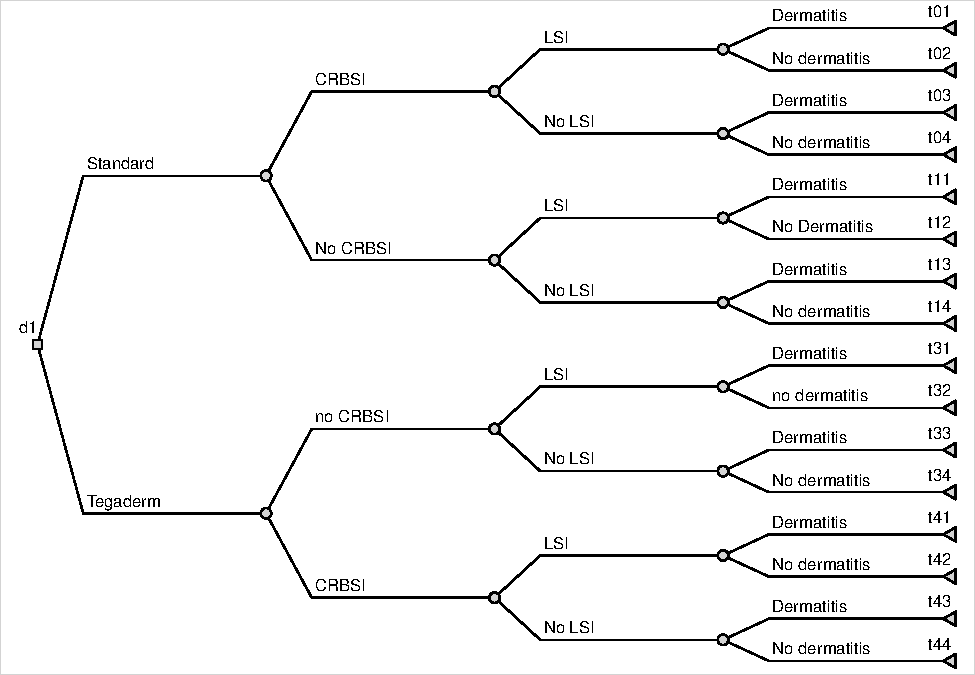
\includegraphics{Sutures_files/figure-latex/draw-1} 

}

\caption{Decision tree for all scenarios.}\label{fig:draw}
\end{figure}

\hypertarget{the-model}{%
\subsection{The model}\label{the-model}}

The decision tree defined by Leaper \emph{et al} {[}1{]} is shown in
figure 1. The model had six input variables: the probability of an SSI
with NCS, the risk ratio of an SSI with TCS compared with NCS, cost of
TCS, cost of NCS, number of sutures per surgical procedure and cost of
an admission with diagnosis of infection. The uncertainties in the
estimates of the variables were described by distributions with
hyperparameters (Table 1).

\begin{longtable}[]{@{}lllrrr@{}}
\caption{Model inputs}\tabularnewline
\toprule
\begin{minipage}[b]{(\columnwidth - 5\tabcolsep) * \real{0.30}}\raggedright
Description\strut
\end{minipage} &
\begin{minipage}[b]{(\columnwidth - 5\tabcolsep) * \real{0.10}}\raggedright
Units\strut
\end{minipage} &
\begin{minipage}[b]{(\columnwidth - 5\tabcolsep) * \real{0.23}}\raggedright
Distribution\strut
\end{minipage} &
\begin{minipage}[b]{(\columnwidth - 5\tabcolsep) * \real{0.12}}\raggedleft
Mean\strut
\end{minipage} &
\begin{minipage}[b]{(\columnwidth - 5\tabcolsep) * \real{0.12}}\raggedleft
Q2.5\strut
\end{minipage} &
\begin{minipage}[b]{(\columnwidth - 5\tabcolsep) * \real{0.12}}\raggedleft
Q97.5\strut
\end{minipage}\tabularnewline
\midrule
\endfirsthead
\toprule
\begin{minipage}[b]{(\columnwidth - 5\tabcolsep) * \real{0.30}}\raggedright
Description\strut
\end{minipage} &
\begin{minipage}[b]{(\columnwidth - 5\tabcolsep) * \real{0.10}}\raggedright
Units\strut
\end{minipage} &
\begin{minipage}[b]{(\columnwidth - 5\tabcolsep) * \real{0.23}}\raggedright
Distribution\strut
\end{minipage} &
\begin{minipage}[b]{(\columnwidth - 5\tabcolsep) * \real{0.12}}\raggedleft
Mean\strut
\end{minipage} &
\begin{minipage}[b]{(\columnwidth - 5\tabcolsep) * \real{0.12}}\raggedleft
Q2.5\strut
\end{minipage} &
\begin{minipage}[b]{(\columnwidth - 5\tabcolsep) * \real{0.12}}\raggedleft
Q97.5\strut
\end{minipage}\tabularnewline
\midrule
\endhead
\begin{minipage}[t]{(\columnwidth - 5\tabcolsep) * \real{0.30}}\raggedright
Excess cost SSI\strut
\end{minipage} &
\begin{minipage}[t]{(\columnwidth - 5\tabcolsep) * \real{0.10}}\raggedright
GBP\strut
\end{minipage} &
\begin{minipage}[t]{(\columnwidth - 5\tabcolsep) * \real{0.23}}\raggedright
Ga(6,500)\strut
\end{minipage} &
\begin{minipage}[t]{(\columnwidth - 5\tabcolsep) * \real{0.12}}\raggedleft
3000\strut
\end{minipage} &
\begin{minipage}[t]{(\columnwidth - 5\tabcolsep) * \real{0.12}}\raggedleft
1101\strut
\end{minipage} &
\begin{minipage}[t]{(\columnwidth - 5\tabcolsep) * \real{0.12}}\raggedleft
5834\strut
\end{minipage}\tabularnewline
\begin{minipage}[t]{(\columnwidth - 5\tabcolsep) * \real{0.30}}\raggedright
P(SSI\textbar NCS)\strut
\end{minipage} &
\begin{minipage}[t]{(\columnwidth - 5\tabcolsep) * \real{0.10}}\raggedright
P\strut
\end{minipage} &
\begin{minipage}[t]{(\columnwidth - 5\tabcolsep) * \real{0.23}}\raggedright
Be(653,6465)\strut
\end{minipage} &
\begin{minipage}[t]{(\columnwidth - 5\tabcolsep) * \real{0.12}}\raggedleft
0.09174\strut
\end{minipage} &
\begin{minipage}[t]{(\columnwidth - 5\tabcolsep) * \real{0.12}}\raggedleft
0.08514\strut
\end{minipage} &
\begin{minipage}[t]{(\columnwidth - 5\tabcolsep) * \real{0.12}}\raggedleft
0.09855\strut
\end{minipage}\tabularnewline
\begin{minipage}[t]{(\columnwidth - 5\tabcolsep) * \real{0.30}}\raggedright
RR(SSI\textbar TCS)\strut
\end{minipage} &
\begin{minipage}[t]{(\columnwidth - 5\tabcolsep) * \real{0.10}}\raggedright
RR\strut
\end{minipage} &
\begin{minipage}[t]{(\columnwidth - 5\tabcolsep) * \real{0.23}}\raggedright
LN(-0.407,0.118)\strut
\end{minipage} &
\begin{minipage}[t]{(\columnwidth - 5\tabcolsep) * \real{0.12}}\raggedleft
0.67\strut
\end{minipage} &
\begin{minipage}[t]{(\columnwidth - 5\tabcolsep) * \real{0.12}}\raggedleft
0.5284\strut
\end{minipage} &
\begin{minipage}[t]{(\columnwidth - 5\tabcolsep) * \real{0.12}}\raggedleft
0.8379\strut
\end{minipage}\tabularnewline
\begin{minipage}[t]{(\columnwidth - 5\tabcolsep) * \real{0.30}}\raggedright
VICRYL plus, pack\strut
\end{minipage} &
\begin{minipage}[t]{(\columnwidth - 5\tabcolsep) * \real{0.10}}\raggedright
GBP\strut
\end{minipage} &
\begin{minipage}[t]{(\columnwidth - 5\tabcolsep) * \real{0.23}}\raggedright
Ga(100,0.036)\strut
\end{minipage} &
\begin{minipage}[t]{(\columnwidth - 5\tabcolsep) * \real{0.12}}\raggedleft
3.63\strut
\end{minipage} &
\begin{minipage}[t]{(\columnwidth - 5\tabcolsep) * \real{0.12}}\raggedleft
2.954\strut
\end{minipage} &
\begin{minipage}[t]{(\columnwidth - 5\tabcolsep) * \real{0.12}}\raggedleft
4.375\strut
\end{minipage}\tabularnewline
\begin{minipage}[t]{(\columnwidth - 5\tabcolsep) * \real{0.30}}\raggedright
Sutures per procedure\strut
\end{minipage} &
\begin{minipage}[t]{(\columnwidth - 5\tabcolsep) * \real{0.10}}\raggedright
n\strut
\end{minipage} &
\begin{minipage}[t]{(\columnwidth - 5\tabcolsep) * \real{0.23}}\raggedright
Ga(200,0.01)\strut
\end{minipage} &
\begin{minipage}[t]{(\columnwidth - 5\tabcolsep) * \real{0.12}}\raggedleft
2\strut
\end{minipage} &
\begin{minipage}[t]{(\columnwidth - 5\tabcolsep) * \real{0.12}}\raggedleft
1.732\strut
\end{minipage} &
\begin{minipage}[t]{(\columnwidth - 5\tabcolsep) * \real{0.12}}\raggedleft
2.287\strut
\end{minipage}\tabularnewline
\begin{minipage}[t]{(\columnwidth - 5\tabcolsep) * \real{0.30}}\raggedright
VICRYL, pack\strut
\end{minipage} &
\begin{minipage}[t]{(\columnwidth - 5\tabcolsep) * \real{0.10}}\raggedright
GBP\strut
\end{minipage} &
\begin{minipage}[t]{(\columnwidth - 5\tabcolsep) * \real{0.23}}\raggedright
Ga(100,0.029)\strut
\end{minipage} &
\begin{minipage}[t]{(\columnwidth - 5\tabcolsep) * \real{0.12}}\raggedleft
2.88\strut
\end{minipage} &
\begin{minipage}[t]{(\columnwidth - 5\tabcolsep) * \real{0.12}}\raggedleft
2.343\strut
\end{minipage} &
\begin{minipage}[t]{(\columnwidth - 5\tabcolsep) * \real{0.12}}\raggedleft
3.471\strut
\end{minipage}\tabularnewline
\bottomrule
\end{longtable}

\hypertarget{results}{%
\subsection{Results}\label{results}}

\begin{longtable}[]{@{}cccccc@{}}
\toprule
\begin{minipage}[b]{(\columnwidth - 5\tabcolsep) * \real{0.28}}\centering
Suture\strut
\end{minipage} &
\begin{minipage}[b]{(\columnwidth - 5\tabcolsep) * \real{0.08}}\centering
Run\strut
\end{minipage} &
\begin{minipage}[b]{(\columnwidth - 5\tabcolsep) * \real{0.19}}\centering
Probability\strut
\end{minipage} &
\begin{minipage}[b]{(\columnwidth - 5\tabcolsep) * \real{0.11}}\centering
Cost\strut
\end{minipage} &
\begin{minipage}[b]{(\columnwidth - 5\tabcolsep) * \real{0.14}}\centering
Benefit\strut
\end{minipage} &
\begin{minipage}[b]{(\columnwidth - 5\tabcolsep) * \real{0.14}}\centering
Utility\strut
\end{minipage}\tabularnewline
\midrule
\endhead
\begin{minipage}[t]{(\columnwidth - 5\tabcolsep) * \real{0.28}}\centering
Antimicrobial\strut
\end{minipage} &
\begin{minipage}[t]{(\columnwidth - 5\tabcolsep) * \real{0.08}}\centering
1\strut
\end{minipage} &
\begin{minipage}[t]{(\columnwidth - 5\tabcolsep) * \real{0.19}}\centering
1\strut
\end{minipage} &
\begin{minipage}[t]{(\columnwidth - 5\tabcolsep) * \real{0.11}}\centering
191.7\strut
\end{minipage} &
\begin{minipage}[t]{(\columnwidth - 5\tabcolsep) * \real{0.14}}\centering
0\strut
\end{minipage} &
\begin{minipage}[t]{(\columnwidth - 5\tabcolsep) * \real{0.14}}\centering
1\strut
\end{minipage}\tabularnewline
\begin{minipage}[t]{(\columnwidth - 5\tabcolsep) * \real{0.28}}\centering
Non-antimicrobial\strut
\end{minipage} &
\begin{minipage}[t]{(\columnwidth - 5\tabcolsep) * \real{0.08}}\centering
1\strut
\end{minipage} &
\begin{minipage}[t]{(\columnwidth - 5\tabcolsep) * \real{0.19}}\centering
1\strut
\end{minipage} &
\begin{minipage}[t]{(\columnwidth - 5\tabcolsep) * \real{0.11}}\centering
281\strut
\end{minipage} &
\begin{minipage}[t]{(\columnwidth - 5\tabcolsep) * \real{0.14}}\centering
0\strut
\end{minipage} &
\begin{minipage}[t]{(\columnwidth - 5\tabcolsep) * \real{0.14}}\centering
1\strut
\end{minipage}\tabularnewline
\bottomrule
\end{longtable}

\hypertarget{tornado-diagram}{%
\subsubsection{Tornado diagram}\label{tornado-diagram}}

\begin{longtable}[]{@{}cccccc@{}}
\caption{Table continues below}\tabularnewline
\toprule
\begin{minipage}[b]{(\columnwidth - 5\tabcolsep) * \real{0.12}}\centering
~\strut
\end{minipage} &
\begin{minipage}[b]{(\columnwidth - 5\tabcolsep) * \real{0.32}}\centering
Description\strut
\end{minipage} &
\begin{minipage}[b]{(\columnwidth - 5\tabcolsep) * \real{0.11}}\centering
Units\strut
\end{minipage} &
\begin{minipage}[b]{(\columnwidth - 5\tabcolsep) * \real{0.13}}\centering
Q2.5\strut
\end{minipage} &
\begin{minipage}[b]{(\columnwidth - 5\tabcolsep) * \real{0.13}}\centering
Q97.5\strut
\end{minipage} &
\begin{minipage}[b]{(\columnwidth - 5\tabcolsep) * \real{0.19}}\centering
outcome.min\strut
\end{minipage}\tabularnewline
\midrule
\endfirsthead
\toprule
\begin{minipage}[b]{(\columnwidth - 5\tabcolsep) * \real{0.12}}\centering
~\strut
\end{minipage} &
\begin{minipage}[b]{(\columnwidth - 5\tabcolsep) * \real{0.32}}\centering
Description\strut
\end{minipage} &
\begin{minipage}[b]{(\columnwidth - 5\tabcolsep) * \real{0.11}}\centering
Units\strut
\end{minipage} &
\begin{minipage}[b]{(\columnwidth - 5\tabcolsep) * \real{0.13}}\centering
Q2.5\strut
\end{minipage} &
\begin{minipage}[b]{(\columnwidth - 5\tabcolsep) * \real{0.13}}\centering
Q97.5\strut
\end{minipage} &
\begin{minipage}[b]{(\columnwidth - 5\tabcolsep) * \real{0.19}}\centering
outcome.min\strut
\end{minipage}\tabularnewline
\midrule
\endhead
\begin{minipage}[t]{(\columnwidth - 5\tabcolsep) * \real{0.12}}\centering
\textbf{1}\strut
\end{minipage} &
\begin{minipage}[t]{(\columnwidth - 5\tabcolsep) * \real{0.32}}\centering
Excess cost SSI\strut
\end{minipage} &
\begin{minipage}[t]{(\columnwidth - 5\tabcolsep) * \real{0.11}}\centering
GBP\strut
\end{minipage} &
\begin{minipage}[t]{(\columnwidth - 5\tabcolsep) * \real{0.13}}\centering
1101\strut
\end{minipage} &
\begin{minipage}[t]{(\columnwidth - 5\tabcolsep) * \real{0.13}}\centering
5834\strut
\end{minipage} &
\begin{minipage}[t]{(\columnwidth - 5\tabcolsep) * \real{0.19}}\centering
31.83\strut
\end{minipage}\tabularnewline
\begin{minipage}[t]{(\columnwidth - 5\tabcolsep) * \real{0.12}}\centering
\textbf{3}\strut
\end{minipage} &
\begin{minipage}[t]{(\columnwidth - 5\tabcolsep) * \real{0.32}}\centering
RR(SSI\textbar TCS)\strut
\end{minipage} &
\begin{minipage}[t]{(\columnwidth - 5\tabcolsep) * \real{0.11}}\centering
RR\strut
\end{minipage} &
\begin{minipage}[t]{(\columnwidth - 5\tabcolsep) * \real{0.13}}\centering
0.5284\strut
\end{minipage} &
\begin{minipage}[t]{(\columnwidth - 5\tabcolsep) * \real{0.13}}\centering
0.8379\strut
\end{minipage} &
\begin{minipage}[t]{(\columnwidth - 5\tabcolsep) * \real{0.19}}\centering
128.3\strut
\end{minipage}\tabularnewline
\begin{minipage}[t]{(\columnwidth - 5\tabcolsep) * \real{0.12}}\centering
\textbf{2}\strut
\end{minipage} &
\begin{minipage}[t]{(\columnwidth - 5\tabcolsep) * \real{0.32}}\centering
P(SSI\textbar NCS)\strut
\end{minipage} &
\begin{minipage}[t]{(\columnwidth - 5\tabcolsep) * \real{0.11}}\centering
P\strut
\end{minipage} &
\begin{minipage}[t]{(\columnwidth - 5\tabcolsep) * \real{0.13}}\centering
0.08514\strut
\end{minipage} &
\begin{minipage}[t]{(\columnwidth - 5\tabcolsep) * \real{0.13}}\centering
0.09855\strut
\end{minipage} &
\begin{minipage}[t]{(\columnwidth - 5\tabcolsep) * \real{0.19}}\centering
82.79\strut
\end{minipage}\tabularnewline
\begin{minipage}[t]{(\columnwidth - 5\tabcolsep) * \real{0.12}}\centering
\textbf{4}\strut
\end{minipage} &
\begin{minipage}[t]{(\columnwidth - 5\tabcolsep) * \real{0.32}}\centering
VICRYL plus, pack\strut
\end{minipage} &
\begin{minipage}[t]{(\columnwidth - 5\tabcolsep) * \real{0.11}}\centering
GBP\strut
\end{minipage} &
\begin{minipage}[t]{(\columnwidth - 5\tabcolsep) * \real{0.13}}\centering
2.954\strut
\end{minipage} &
\begin{minipage}[t]{(\columnwidth - 5\tabcolsep) * \real{0.13}}\centering
4.375\strut
\end{minipage} &
\begin{minipage}[t]{(\columnwidth - 5\tabcolsep) * \real{0.19}}\centering
90.67\strut
\end{minipage}\tabularnewline
\begin{minipage}[t]{(\columnwidth - 5\tabcolsep) * \real{0.12}}\centering
\textbf{6}\strut
\end{minipage} &
\begin{minipage}[t]{(\columnwidth - 5\tabcolsep) * \real{0.32}}\centering
VICRYL, pack\strut
\end{minipage} &
\begin{minipage}[t]{(\columnwidth - 5\tabcolsep) * \real{0.11}}\centering
GBP\strut
\end{minipage} &
\begin{minipage}[t]{(\columnwidth - 5\tabcolsep) * \real{0.13}}\centering
2.343\strut
\end{minipage} &
\begin{minipage}[t]{(\columnwidth - 5\tabcolsep) * \real{0.13}}\centering
3.471\strut
\end{minipage} &
\begin{minipage}[t]{(\columnwidth - 5\tabcolsep) * \real{0.19}}\centering
88.25\strut
\end{minipage}\tabularnewline
\begin{minipage}[t]{(\columnwidth - 5\tabcolsep) * \real{0.12}}\centering
\textbf{5}\strut
\end{minipage} &
\begin{minipage}[t]{(\columnwidth - 5\tabcolsep) * \real{0.32}}\centering
Sutures per procedure\strut
\end{minipage} &
\begin{minipage}[t]{(\columnwidth - 5\tabcolsep) * \real{0.11}}\centering
n\strut
\end{minipage} &
\begin{minipage}[t]{(\columnwidth - 5\tabcolsep) * \real{0.13}}\centering
1.732\strut
\end{minipage} &
\begin{minipage}[t]{(\columnwidth - 5\tabcolsep) * \real{0.13}}\centering
2.287\strut
\end{minipage} &
\begin{minipage}[t]{(\columnwidth - 5\tabcolsep) * \real{0.19}}\centering
89.52\strut
\end{minipage}\tabularnewline
\bottomrule
\end{longtable}

\begin{longtable}[]{@{}cc@{}}
\toprule
\begin{minipage}[b]{(\columnwidth - 1\tabcolsep) * \real{0.12}}\centering
~\strut
\end{minipage} &
\begin{minipage}[b]{(\columnwidth - 1\tabcolsep) * \real{0.19}}\centering
outcome.max\strut
\end{minipage}\tabularnewline
\midrule
\endhead
\begin{minipage}[t]{(\columnwidth - 1\tabcolsep) * \real{0.12}}\centering
\textbf{1}\strut
\end{minipage} &
\begin{minipage}[t]{(\columnwidth - 1\tabcolsep) * \real{0.19}}\centering
175.1\strut
\end{minipage}\tabularnewline
\begin{minipage}[t]{(\columnwidth - 1\tabcolsep) * \real{0.12}}\centering
\textbf{3}\strut
\end{minipage} &
\begin{minipage}[t]{(\columnwidth - 1\tabcolsep) * \real{0.19}}\centering
43.11\strut
\end{minipage}\tabularnewline
\begin{minipage}[t]{(\columnwidth - 1\tabcolsep) * \real{0.12}}\centering
\textbf{2}\strut
\end{minipage} &
\begin{minipage}[t]{(\columnwidth - 1\tabcolsep) * \real{0.19}}\centering
96.07\strut
\end{minipage}\tabularnewline
\begin{minipage}[t]{(\columnwidth - 1\tabcolsep) * \real{0.12}}\centering
\textbf{4}\strut
\end{minipage} &
\begin{minipage}[t]{(\columnwidth - 1\tabcolsep) * \real{0.19}}\centering
87.83\strut
\end{minipage}\tabularnewline
\begin{minipage}[t]{(\columnwidth - 1\tabcolsep) * \real{0.12}}\centering
\textbf{6}\strut
\end{minipage} &
\begin{minipage}[t]{(\columnwidth - 1\tabcolsep) * \real{0.19}}\centering
90.5\strut
\end{minipage}\tabularnewline
\begin{minipage}[t]{(\columnwidth - 1\tabcolsep) * \real{0.12}}\centering
\textbf{5}\strut
\end{minipage} &
\begin{minipage}[t]{(\columnwidth - 1\tabcolsep) * \real{0.19}}\centering
89.11\strut
\end{minipage}\tabularnewline
\bottomrule
\end{longtable}

\begin{figure}

{\centering \includegraphics{Sutures_files/figure-latex/tornado-1} 

}

\caption{Tornado chart showing mean cost savings per procedure.}\label{fig:tornado}
\end{figure}

\hypertarget{references}{%
\section*{References}\label{references}}
\addcontentsline{toc}{section}{References}

\hypertarget{refs}{}
\begin{CSLReferences}{0}{0}
\leavevmode\hypertarget{ref-leaper2017}{}%
\CSLLeftMargin{1 }
\CSLRightInline{Leaper DJ, Edmiston Jr CE, Holy CE. Meta-analysis of the
potential economic impact following introduction of absorbable
antimicrobial sutures. \emph{{BJS} (British Journal of Surgery)}
2017;\textbf{104}:e134--44.
doi:\href{https://doi.org/10.1002/bjs.10443}{10.1002/bjs.10443}}

\end{CSLReferences}

\end{document}
